
\begin{figure}[H]
    \centering
    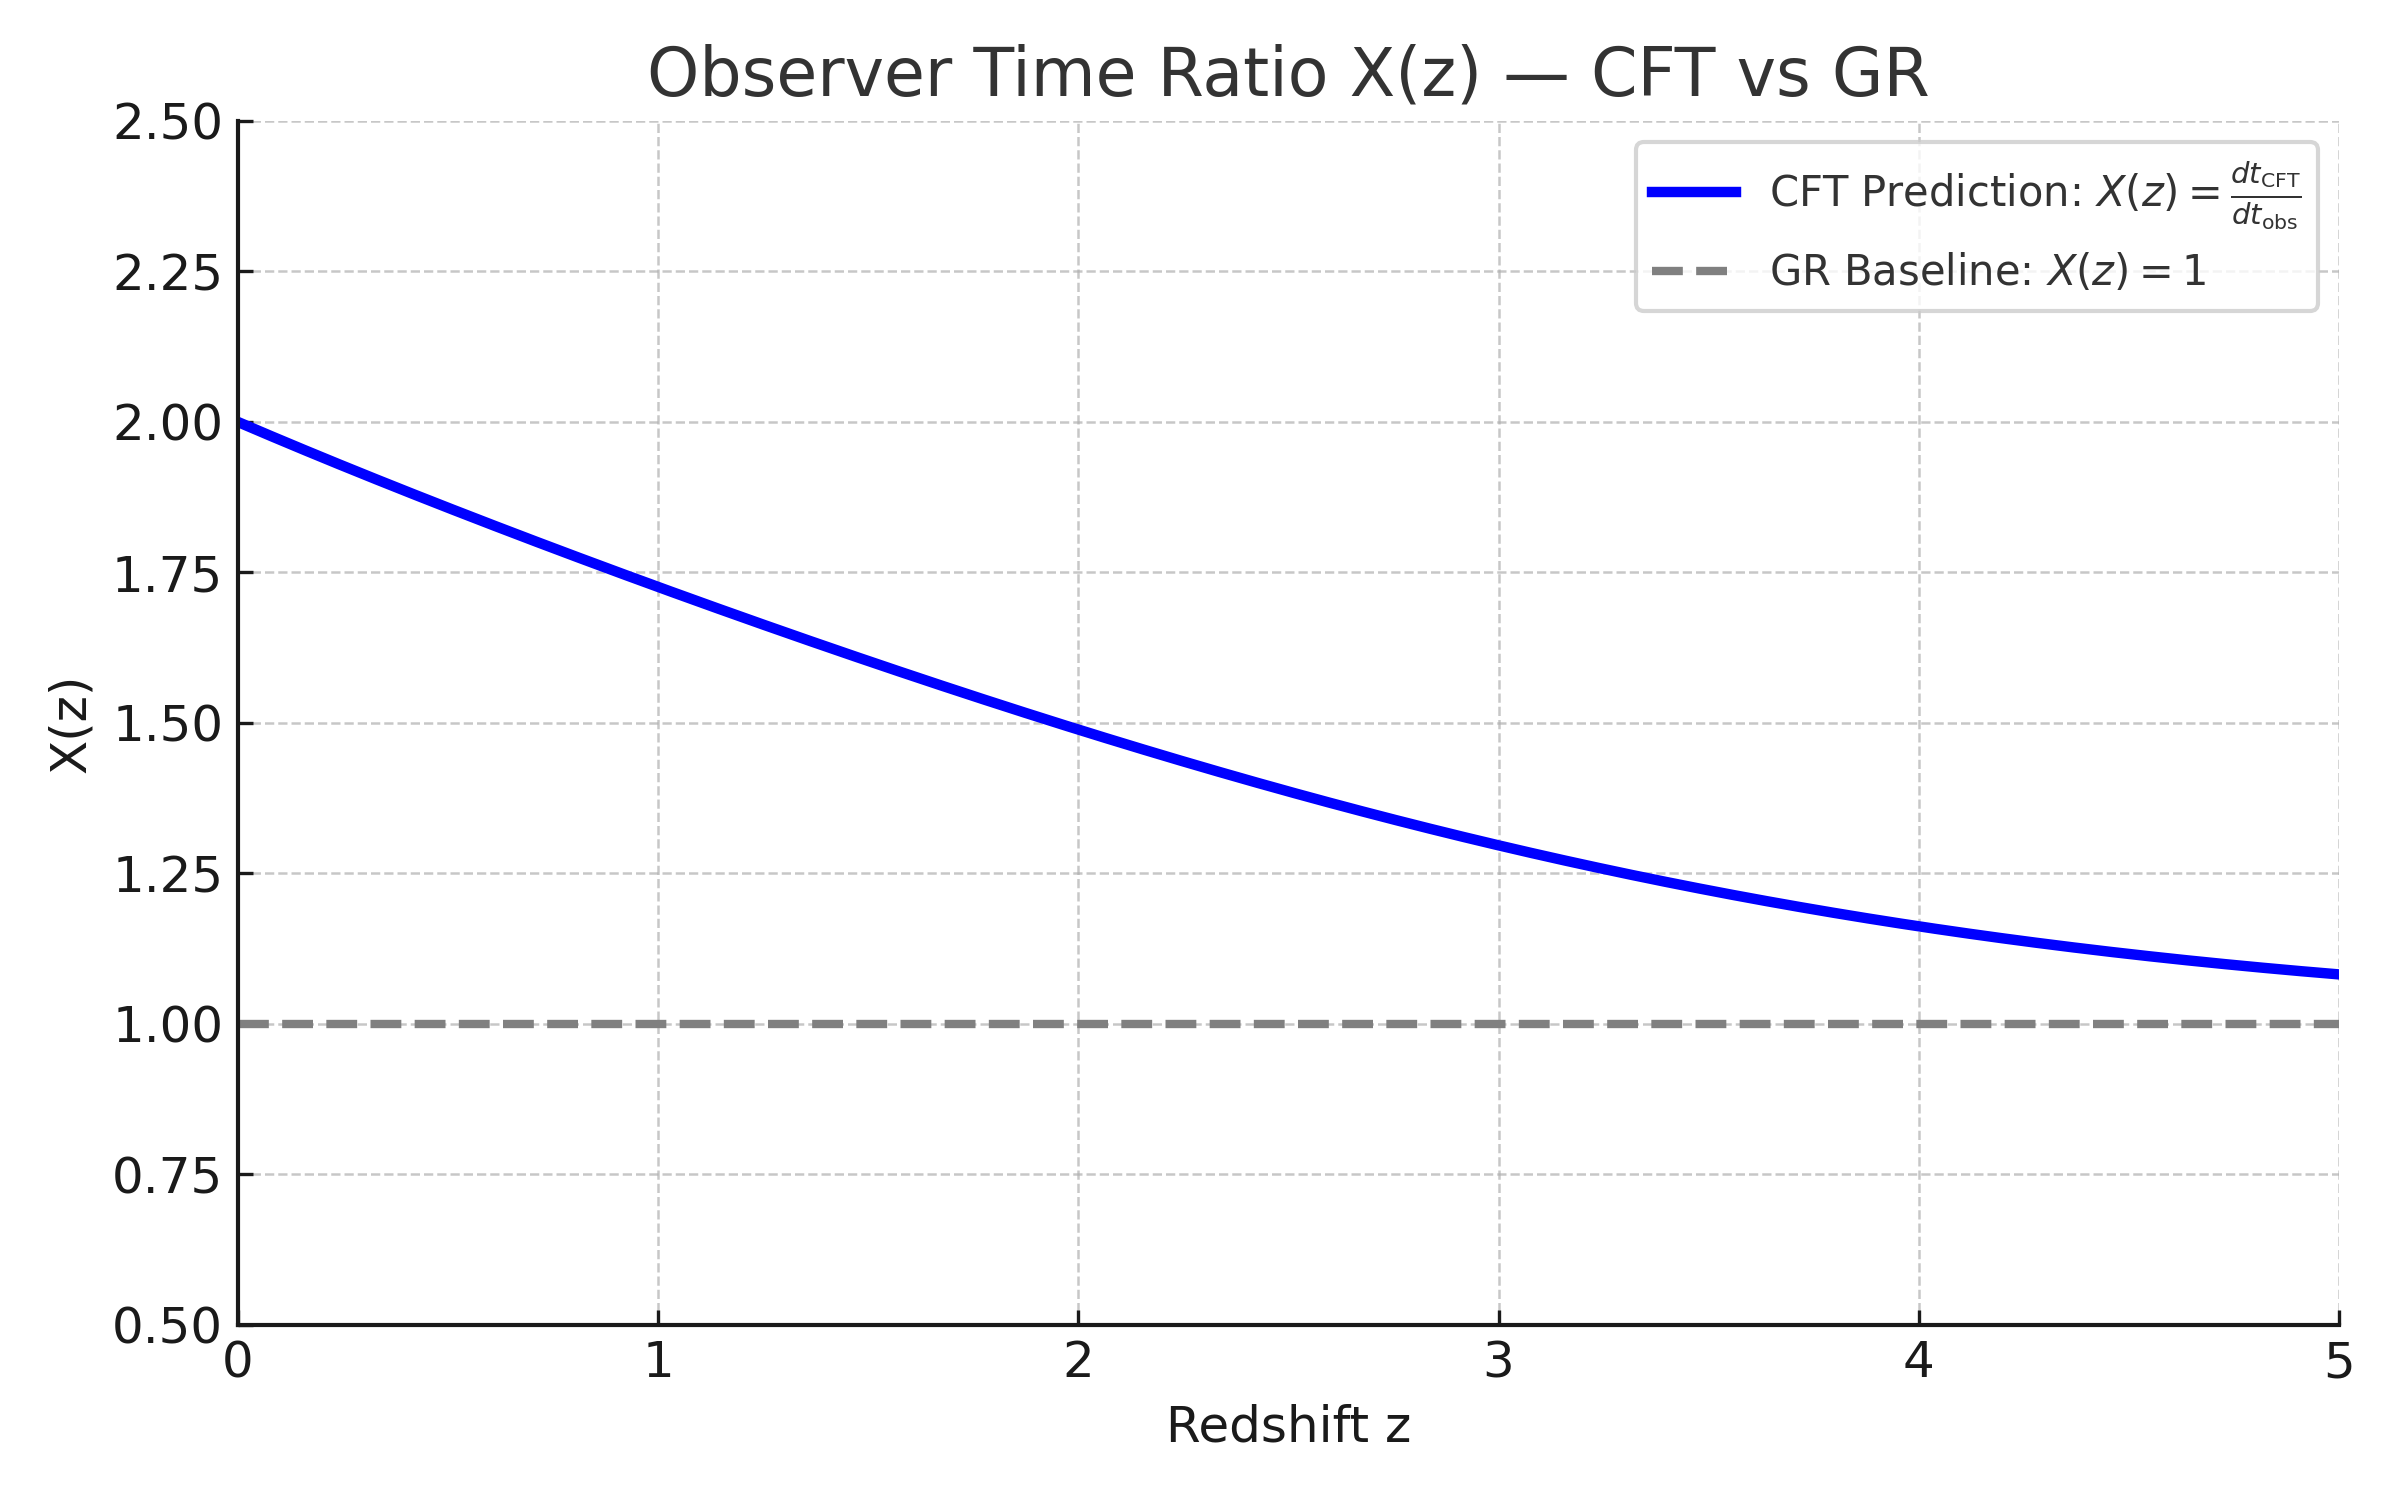
\includegraphics[width=0.9\textwidth]{Xz_CFT_vs_GR.png}
    \caption{Observer Time Ratio $X(z)$ comparing Chronotension Field Theory (CFT) and General Relativity (GR). CFT predicts a divergence between cosmic and observer time, with $X(z) > 1$ at high redshift. GR assumes $X(z) = 1$. This supports CFT's remapping approach as key to resolving discrepancies in $H(z)$ and other observables.}
\end{figure}
